
{\rmfamily
This work was previously published in ACM SIGCHI 2016 \cite{ka} and has been adapted for this document.
}

\begin{figure}
    \centering
    \frame{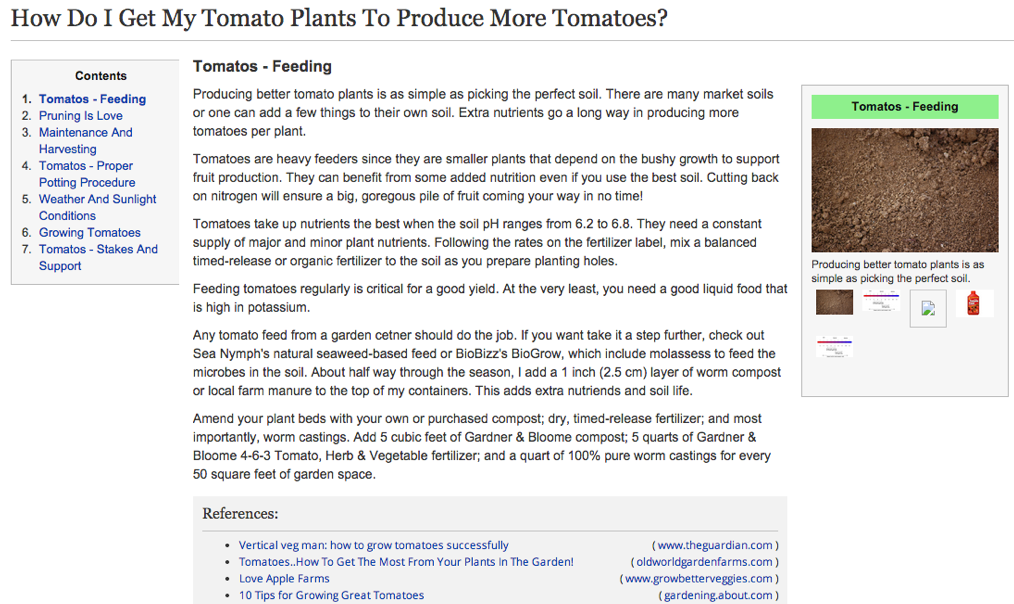
\includegraphics[width=1\columnwidth]{Chapters/KA/final_answer}}
    \caption[Alloy clusters synthesized into a report articles using the Knowledge Accelerator.]{Example report synthesized by the Knowledge Accelerator system. The table of content on the left listed cluster names generated from Alloy, each corresponded to a different section in the report.}
    \label{fig:final_answer}
\end{figure}

\begin{figure}
    \centering
    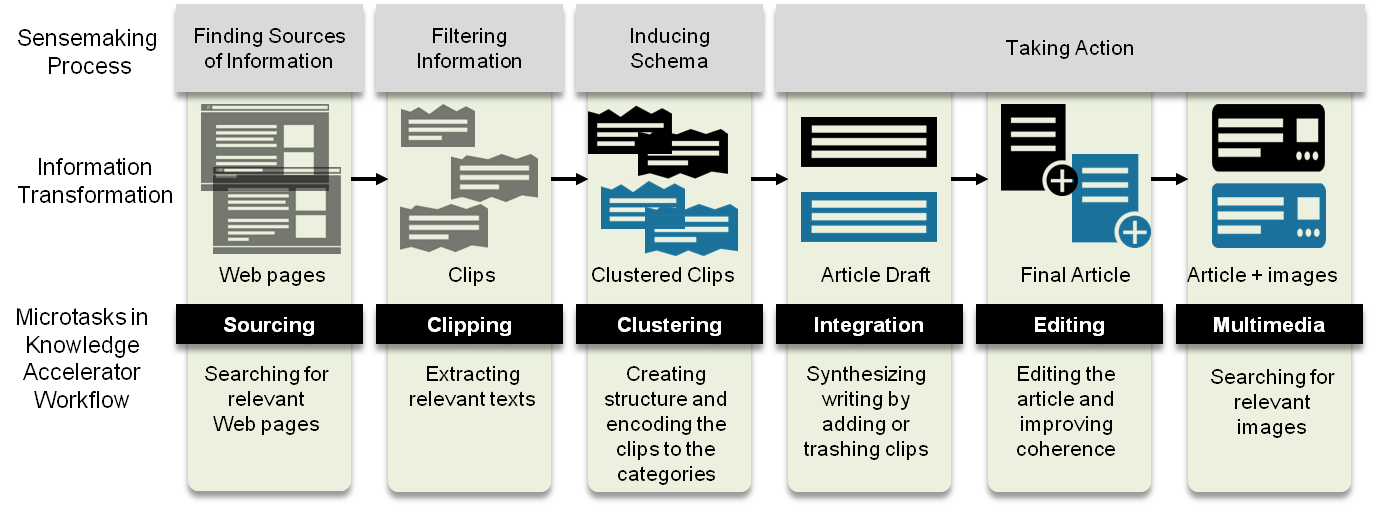
\includegraphics[width=1\columnwidth]{Chapters/KA/overview}
    \caption[The Knowledge Accelerator (KA) with Alloy as the Clustering Stage.]{The process of the Knowledge Accelerator (KA). Alloy is used for the Clustering Stage of the pipeline.}
    \label{fig:process}
\end{figure}


To evaluate the usefulness of structures generated by Alloy in a more realistic scenarios, we first used Alloy to clusters a larger set of information seeking datasets (Table~\ref{tab:evaluation}) collected using the same procedure as described in \cref{chap:info_seek_datasets}. We then developed a prototype system called the ``Knowledge Accelerator'' (KA) to synthesize the output of Alloy into articles. Each of the cluster produced by Alloy corresponds to a different section in an article. An example of the output of the system for the target question ``How do I get my tomato plants to produce more tomatoes?'' can be found in Figure~\ref{fig:final_answer}.

In addition, the KA system probes how to accomplish a complex information synthesis task entirely through relatively small contributions. We limited our maximum task payment to \$1 US, aimed at incentivizing a Target task time of approximately 5-10 minutes. Critically, the KA system accomplishes this process without a core overseer or moderator. Figure \ref{fig:process} shows the overview of the KA System with Alloy being the Clustering Stage. For more details on the KA system refer to \cite{ka}.

We evaluated the usefulness and coherence of the articles by comparing them against webpages an individual might use if they were to complete the same tasks without KA and Alloy --- Top Google search results that consists of expert-written articles published by trusted sources such as CDC.gov or the New York Times, as well as popular online forums such as TripAdvisor and Yahoo Answers.

\subsection{Experimental Settings}

Eleven topics were selected for evaluation by browsing question and answer forums, Reddit.com, and referencing online browsing habits \cite{pewReport}. For questions Q3 and Q8 we added additional constraints (i.e., having kids and age) to test the performance of the system for more personalized questions.
To compare the two conditions, participants were recruited through the Amazon Mechanical Turk US-only pool and paid \$1.50 for rating two webpages. Each participant was randomly assigned an output article from KA and a top search result webpage for the same topic (Figure~\ref{fig:aggregated}), and rate both webpages based on six criteria using 7-point Likert scale questions and provided free-form explanations: \emph{comprehensiveness}, \emph{confidence}, \emph{helpfulness}, \emph{trustworthiness}, \emph{understandability}, and \emph{writing}. We averaged ratings on these dimensions into a single score representing the overall perceived quality of the page.


\begin{table}
  \centering
  \footnotesize
% question, number of sources, number of clips, number of turkers
  \begin{tabular}{l r l}

	Question &
	\multicolumn{1}{c}{N} &
    \multicolumn{1}{c}{Score} \\
    \hline
	% 102
	\multicolumn{1}{p{0.75\columnwidth}}{\textbf{Q1}: \textit{How do I unclog my bathtub drain?}}
	& 116 & ~0.292 * \\

	% 115	
	\multicolumn{1}{p{0.75\columnwidth}}{\textbf{Q2}: \textit{How do I get my tomato plants to produce more tomatoes?}}
	& 177 & ~0.420 * \\

	% 153
	\multicolumn{1}{p{0.75\columnwidth}}{\textbf{Q3}: \textit{What are the best attractions in LA if I have two little kids?}}
	& 158 & -0.044 \\

	% 116
	\multicolumn{1}{p{0.75\columnwidth}}{\textbf{Q4}: \textit{What are the best day trips possible from Barcelona, Spain?}}
	& 98 & -0.109 \\

	% 177
	\multicolumn{1}{p{0.75\columnwidth}}{\textbf{Q5}: \textit{My Worcester CDi Boiler pressure is low. How can I fix it?}}
	& 139 & ~0.878 * \\

	% 168
	\multicolumn{1}{p{0.75\columnwidth}}{\textbf{Q6}: \textit{2003 Dodge Durango has an OBD-II error code of P440. How do I fix it?}}
	& 138 & ~0.662 * \\

	% 175
	\multicolumn{1}{p{0.75\columnwidth}}{\textbf{Q7}: \textit{2005 Chevy Silverado has an OBD-II error code of C0327. How do I fix it?}}
	& 135 & ~0.412 * \\

    % 160
	\multicolumn{1}{p{0.75\columnwidth}}{\textbf{Q8}: \textit{How do I deal with the arthritis in my knee as a 28 year old?}}
	& 139 & ~0.391 * \\

    % 161
	\multicolumn{1}{p{0.75\columnwidth}}{\textbf{Q9}: \textit{My Playstation 3 has a solid yellow light, how do I fix it?}}
	& 119 & ~0.380 * \\

    % 162
	\multicolumn{1}{p{0.75\columnwidth}}{\textbf{Q10}: \textit{What are the key arguments for and against Global Warming?}}
	& 138 & ~0.386 * \\

    % 163
	\multicolumn{1}{p{0.75\columnwidth}}{\textbf{Q11}: \textit{How do I use the VIM text editor?}}
	& 138 & ~0.180 \\
    \hline
    \multicolumn{3}{l}{\textbf{*} = significant at $p < 0.01$ after Bonferroni correction}\\

  \end{tabular}
  \caption[Comparing KA output with top websites for the eleven questions.]{Average difference between the KA output and top websites for the eleven questions (positive indicates higher ratings for KA, negative indicates higher ratings for the competing website). Each rating was an aggregate of 6 questions on a 7-point Likert scale.}
  \label{tab:evaluation}
\end{table}

\begin{figure}
    \centering
    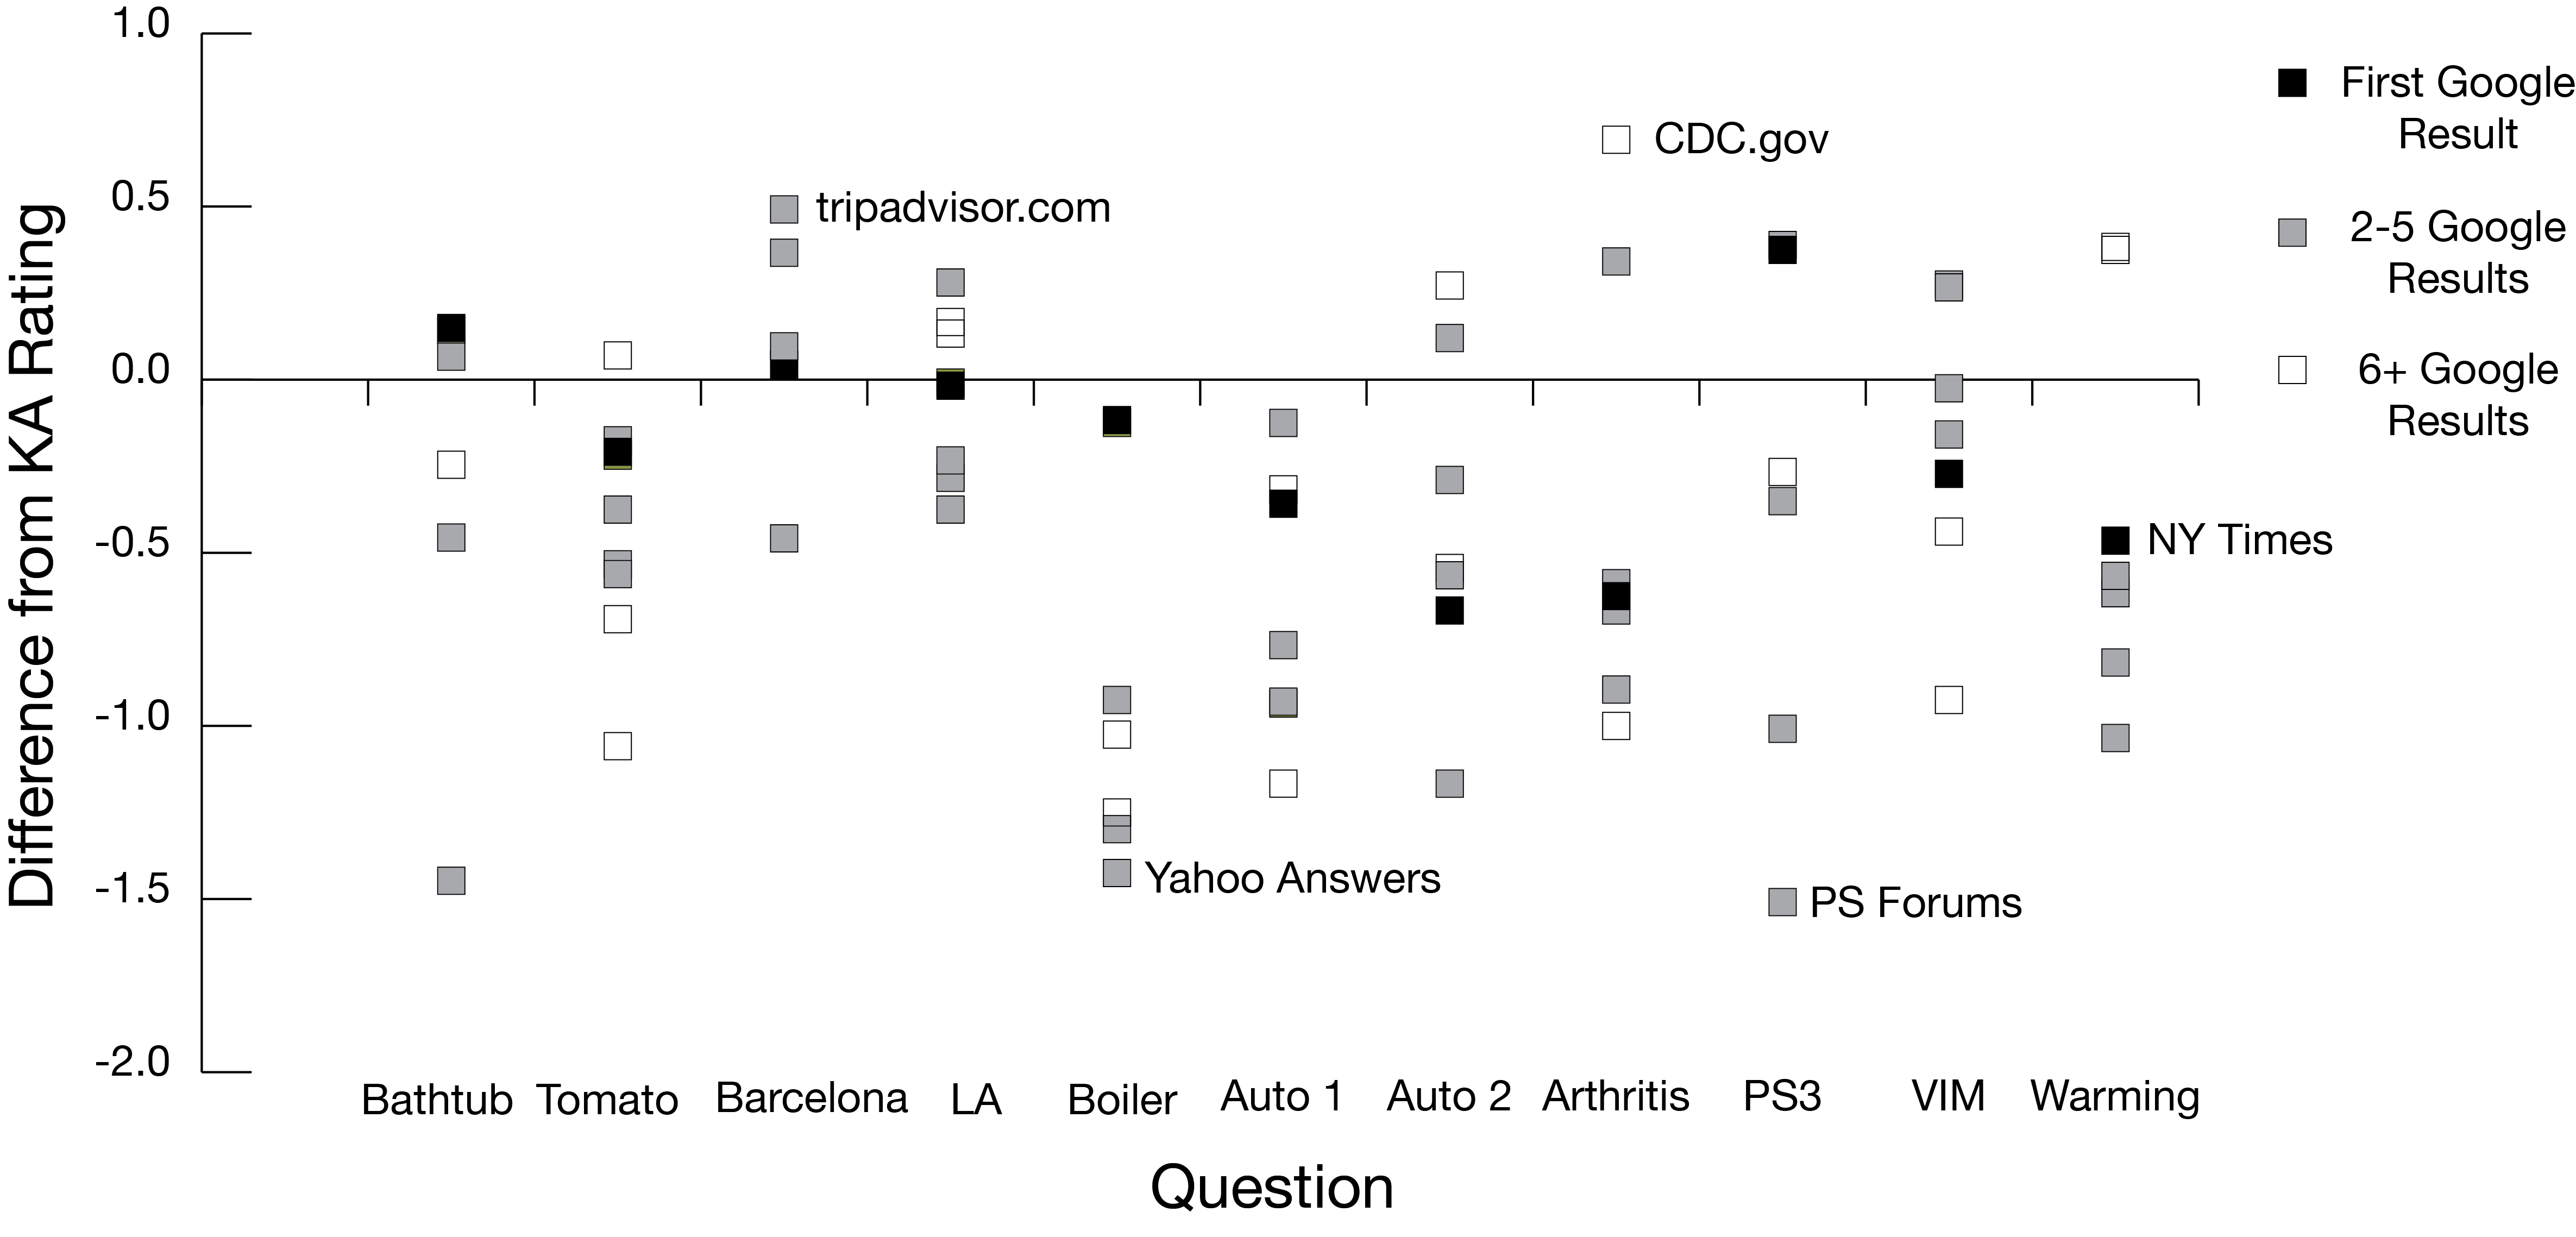
\includegraphics[width=1\columnwidth]{Chapters/KA/source_eval_graph}
    \caption[Results across questions and websites.]{Results across questions and websites. Points represent the average aggregate score difference between the KA answer and an existing site}
    \label{fig:aggregated}
\end{figure}

\subsection{Results}

\begin{table}
  \centering
  \small
% question, number of sources, number of clips, number of turkers
  \begin{tabular}{lrrr}
    \hline
    \textbf{Phase} & \textbf{Task Pay} & \textbf{Avg. \# of Tasks} & \textbf{Avg. Cost} \\
    \hline
	Sourcing & \$0.25 & 15 & \$3.75 \\

    Clipping & \$0.50 & 21.6 & \$10.80 \\

    Alloy Head Cast & \$1.00 & 10 & \$10.00 \\

    Alloy Merge + Tail Cast & \$1.00 & 10 & \$10.00 \\

    Integrate & \$0.50 & 37.2 & \$18.60 \\

    Edit 1 & \$0.75 & 28.8 & \$21.60 \\

    Edit 2 & \$1.00 & 28.8 & \$28.80 \\

    Images & \$0.50 & 9 & \$4.50 \\
    \hline    
    \textbf{Total} & & 160.4 & \$108.05 \\
    \hline
  \end{tabular}
  \caption[Average number of worker tasks and cost of running KA.]{Average number of worker tasks and average cost per phase, and overall, to run a question.}
  \label{tab:cost}
\end{table}

The costs of running a question through the KA system is shown in Table~\ref{tab:cost}. Across the 11 topics we tested, a full run with around 100 short text clips costed an average of \$108.50, of which around \$15 is spent on searching and extracting the text clips from webpages, \$20.00 is spent by the Alloy system, and the rest on synthesizing each of the Alloy clusters into a section in the final article and making sure the different sections are coherent.

Aggregating across all questions, KA output was rated significantly higher than the top 5 Google results (KA: $\bar{x} = 2.904$ vs Alt. Sites: $\bar{x} = 2.545$, $t(1493) = 13.062$, $p < 0.001$). An analysis of individual questions corrected for multiple comparisons is shown in Table~\ref{tab:evaluation}. 

The strongly positive results found were surprising because some of the websites in the comparison set were written by experts and had well-established reputations. Only on the two travel questions, Barcelona ($\bar{x} = -0.109$) and LA ($\bar{x} = -0.044$), and the VIM question ($\bar{x} = 0.180$) did the KA output not significantly outperform the comparison pages. A closer examination of these pages suggests that for the two travel questions, because of the strong internet commodity market surrounding travel, a considerable amount of effort has been spent on curating good travel resources. Even with the slightly more specific LA query, there were still two specialized sites dedicated to attraction for kids in LA (Mommypoppins.com and ScaryMommy.com). The VIM question represented a mismatch between our output and the question style. A number of the sources for the question were tutorials, however in the clipping phase, these ordered tutorials were broken up into unordered clips, creating an information model breakdown. This points out an interesting limitation in the KA approach, and suggests that adding support for more structured answers (e.g., including sequential steps) could be valuable future work. 


%As an additional external evaluation, for the two questions (Q6 and Q7) related to automotive systems we compared the discovered categories from the KA system with two commercial knowledge service products generated by expert technicians. We compared the KA response's accuracy and comprehensiveness, and found that it discovered all the categories referred to in these two commercial products for each question. Furthermore, the categories from the KA output provided more categories not mentioned in the commercial product (average 2.5 categories from two commercial products, while average 9.5 categories from KA). We validated these additional categories with expert automotive professionals who evaluated them as also being plausible and reasonable for the given questions. There was one instance in which two distinct categories (Encoder Motor and Encoder Motor Sensor) from the commercial products were clustered into the single category named Encoder Motor Assembly in the KA output. However, the full text answer from the KA system for Encoder Motor Assembly did still contain these two sub-components with different repair procedures. 

%It may seem surprising that KA would work well for questions such as automotive error codes, where the response relies heavily on technical knowledge and jargon. On further inspection we believe this is because there are many online resources that have valuable information pertaining to these questions but are in unstructured and dialog oriented forms. Workers in the sourcing phase found rich sources of online information from many car enthusiast discussion forums, in which members tried to diagnose and help each other solve their automative problems. Although crowd workers may not understand the esoteric jargon of the automative domain, their understanding of grammar, semantics, and argument structure was sufficient to let them find, filter, cluster, integrate, and edit this domain-specific information. These results suggest a interesting avenue for future research leveraging human understanding of semantics and argument structure to extend crowdsourcing to process expert domain knowledge and to understand the limits of where such an approach breaks down.

%(see Figure~\ref{fig:feedback})



%\subsection{Discussion}

 \begin{figure}
 	\fbox{ \vbox{
 		\ttfamily
 		\footnotesize
 		
		\textbf{categories induced during clipping (without Alloy):}\\
 		Boil Water, use hot water, Plunger, try a snake, How to Remove drain stopper, bleach, Use Drano Max Gel, baking soda, drain, tips to unclog, problem, tools, research, internet research, ..., etc.
 		
 		\rule{\columnwidth}{0.1pt}
 		
 		\textbf{categories induced by Alloy:}\\
 		Hot Water, Plunge, Plunger, Snake the Drain, Remove the Drain Cover, Drain Cleaner, Remove Hair Clusters.
 		
 		\rule{\columnwidth}{0.1pt}
 		
 		\textbf{gold-standard categories:}\\
 		Hot Water, Plunger, Plumbing Snake, Remove Cover, Chemicals, Bent Wire Hanger, Call a Plumber, Shop Vacuum.
 	}}
 	\caption[Categories induced from different stages of KA.]{Categories induced from different stages for Q1: \textit{How do I unclog my bathtub drain?}}
 	\label{fig:delayed-structuring}
 \end{figure}

The strong performance of the system is perhaps surprising given that its output was generated by many non-expert crowd workers, none of whom saw the big picture of the whole, and Alloy is a core component that provided useful and coherent structures for producing the final report. Initially we had workers provide labels to categorize each clip, which we planned to use to develop a structure for the article. However, the lack of context of the bigger picture made these labels poorly suited for inducing a good structure. For example, in Figure~\ref{fig:delayed-structuring} the top box shows the category structure induced by crowdworkers during clipping and without using Alloy during clipping, categories induced using Alloy, and gold standard categories developed by two independent annotators with access to all clips and sources, respectively. Categories induced without using Alloy matched poorly with the gold standard categories, and include categories with very different abstraction levels (e.g., \textit{Use Drano Max Gel} vs \textit{tips}). On the other hand, Alloy produced categories that were more coherent and matched more with gold-standard categories.

While we do not believe that this should be interpreted as a replacement for expert creation and curation of content, instead, the power of the system may actually be attributable to the value created by those experts by generating content which the crowd workers could synthesize and structure into a coherent digest. This explanation suggests that the approach would be most valuable where experts generate a lot of valuable information that is unstructured and redundant, such as the automative questions in which advice from car enthusiasts was spread across many unstructured discussion forums. In contrast, KA's output did not outperform top web sources for topics such as travel, where there are heavy incentives for experts to generate well structured content.  We believe its performance is likely due to its aggregation of multiple expert viewpoints rather than particularly excellent writing or structure per se, never the less, the KA system showcased that the structures produced by Alloy can be synthesized into coherent articles that were useful for exploratory searchers.

